%==============================================================================
% DecisionGPT -- IEEE conference-format manuscript
%
% Generated by converting docs/PAPER_DRAFT.md (the finalized, audited manuscript)
% to IEEEtran two-column format. NO scientific content was changed during this
% conversion: every numerical value, confidence interval, Wilcoxon result,
% effect size, wins/ties/losses count, predictive metric and causal-recovery
% metric is carried over verbatim from the finalized manuscript, which in turn
% reads them from the frozen experiment manifest
% (experiments/experiment_manifest.json,
%  SHA-256 94aa419c703b1babb465975463b26e55255755a7687ecbecadb6db4c4c15cbff).
%
% No experiment was run, re-run, re-seeded or modified. R0/D0 unchanged.
% R3 remains NOT PROMOTED. Real SME outcomes = 0. PredictionEvaluation = 0.
% The real-world decision-outcome validation table (\ref{tab:table2}) remains
% NOT READY. Real LLM remains BLOCKED. CAUSALLY_VALIDATED = 0.
% (LaTeX assigns table/figure numbers automatically in order of appearance;
%  every reference in the text uses \ref, so numbers resolve correctly.)
%
% Compile:  latexmk -pdf main.tex        (or:  pdflatex; bibtex; pdflatex x2)
% Requires: IEEEtran.cls + IEEEtran.bst (standard in TeX Live / MiKTeX / Overleaf)
%           and: graphicx, amsmath, amssymb, array, booktabs, url, hyperref
%==============================================================================
\documentclass[conference]{IEEEtran}
\IEEEoverridecommandlockouts

\usepackage[T1]{fontenc}
\usepackage{graphicx}
\usepackage{amsmath}
\usepackage{amssymb}
\usepackage{array}
\usepackage{booktabs}
\usepackage{url}
\usepackage[hidelinks]{hyperref}

\graphicspath{{figures/}}

% ---- convenience macros for frequently repeated code-style tokens ------------
\newcommand{\code}[1]{\texttt{#1}}
\newcommand{\Nnz}{N_{\neq}}                 % number of non-zero paired differences
\newcommand{\rzn}{r=Z/\sqrt{\Nnz}}
\newcommand{\expid}[1]{\texttt{#1}}

\begin{document}

\title{Does a Multi-Agent Layer Help? A Controlled Component-Level Evaluation of
an Integrated Decision-Support Architecture for Data-Constrained SMEs}

%------------------------------------------------------------------------------
% AUTHOR BLOCK  (author-block decisions resolved by the project)
%
%   * Author list and order (verbatim as supplied):
%       1. K. S. Sri Vardhan   2. R Rohit   3. K. Rahul   4. Felix
%     All four: SCOPE, VIT-AP University, Vijayawada, Andhra Pradesh, India.
%   * Corresponding author: K. S. Sri Vardhan (vardhan.23bce8389@vitapstudent.ac.in)
%     -- noted via \thanks below.
%   * Prof. Yelepi Usha Rani: supervisor/guide INFORMATION ONLY. She is NOT a
%     co-author and is NOT in the author list. Her exact name/affiliation/email
%     (as supplied) appear only in the supervisor \thanks note below.
%   * Student registration numbers: NOT included (per instruction).
%   * ORCID / funding / other acknowledgements: none.
%------------------------------------------------------------------------------
\author{%
\IEEEauthorblockN{K. S. Sri Vardhan, R Rohit, K. Rahul, and Felix}
\IEEEauthorblockA{SCOPE, VIT-AP University, Vijayawada, Andhra Pradesh, India\\
vardhan.23bce8389@vitapstudent.ac.in, rohit.23bce8394@vitapstudent.ac.in,\\
rahul.23bce8396@vitapstudent.ac.in, felix.23bce8402@vitapstudent.ac.in}
\thanks{Corresponding author: K. S. Sri Vardhan
(vardhan.23bce8389@vitapstudent.ac.in).}
\thanks{Supervisor: Prof. Yelepi Usha Rani, Professor, SCOPE, VIT-AP University,
Vijayawada, Andhra Pradesh, India (usharani.y@vitap.ac.in).}
}

\maketitle

%==============================================================================
\begin{abstract}
This paper reports a controlled, synthetic-scenario evaluation of an integrated
decision-support architecture; it does not evaluate the system on real
businesses, and no real small- or medium-enterprise (SME) decision outcomes were
available at any point in the study. Within that scope, we ask which components
of a goal-to-strategy decision-support pipeline carry measurable value, and
whether adding a rule-based multi-agent evaluation layer improves simulated
decision quality beyond a deterministic business decision-simulation layer.
Using a pre-registered design of 12 deliberately constructed scenarios crossed
with 5 random seeds (60 paired observations per configuration), we find that the
decision-simulation layer is the only component that raises a simulated
goal-attainment metric (from a mean of $0.000$ for a prediction-only pipeline to
$0.486$ with the simulation layer), and that adding the implemented three-agent
rule-based evaluation layer on top of it \emph{reduces} the metric to $0.084$
(paired Wilcoxon signed-rank $p<10^{-4}$; 45 of 60 paired observations worse,
none better; mean shift $-0.401$, 95\% CI $[-0.478,-0.324]$). A component
ablation attributes the entire measurable objective effect to the simulation
layer; removing the association-graph, multi-agent, explanation, or memory
components changes the objective by exactly $0.000$. Trace analysis localises
the degradation to the optimizer's unbounded risk-penalty term acting on a
mis-scaled extrapolation-risk heuristic: neutralising that single term recovers
the metric to $0.583$, and the term is decisive in 75\% of paired cases
($0/390$ risk-score transmission errors). A pre-registered recalibration of the
risk heuristic improves the synthetic metric to $0.168$ (mean shift $+0.083$,
$p=0.025$, 5 of 60 non-zero pairs) but is inert on the one real Indian price
dataset available and is \emph{not adopted}; production retains the original
configuration. Predictive sub-components (forecasting, churn) and a synthetic
causal-recovery method validation behave as expected on their datasets. We make
no claim of real-world effectiveness, no real-LLM evaluation was performed, and
no causal effect is established (\code{CAUSALLY\_VALIDATED = 0}). The
contribution is a reproducible component-level evaluation protocol, a
mechanism-diagnosed negative result for the tested multi-agent configuration,
and an evidence-boundary framework that separates controlled synthetic evidence
from the real-world validation that remains future work. The full manifest,
data-category separation, and clean-room reproduction are released.
\end{abstract}

\begin{IEEEkeywords}
decision-support systems, prescriptive analytics, controlled evaluation,
component ablation, multi-agent systems, negative results, simulation-based
decision support, risk-aware optimization, reproducibility, pre-registration
\end{IEEEkeywords}

%==============================================================================
\section{Introduction}
\label{sec:intro}

Small and medium enterprises (SMEs) operate under acute data constraints ---
limited historical records, no analytics staff, and uncertain returns on
analytics investment~\cite{OECD2021}. In the Indian micro, small and medium
enterprise (MSME) sector specifically, a large share of activity is informal,
with limited financial records and little credit history, which impedes formal
data integration and digital adoption~\cite{Buteau2021}. Business-intelligence
and predictive-analytics tools describe what happened and forecast what may
happen, but stop short of recommending an action toward a stated goal;
prescriptive analytics names this gap and its reviews note a persistent shortage
of controlled empirical evaluation of end-to-end
pipelines~\cite{Lepenioti2020,Arnott2014,Shmueli2011}.

A common response is to compose more capability into one architecture:
forecasting, what-if simulation, risk scoring, contextual or causal
information, memory, explanation, and --- increasingly --- multiple reasoning
agents that debate a recommendation. Multi-agent debate has been reported to
improve reasoning and factuality on question-answering and reasoning
benchmarks~\cite{Du2023,Liang2024,Li2024}. A growing counter-literature,
however, finds that added agents do not reliably help: a single agent with a
strong prompt can match multi-agent discussion~\cite{Wang2024}, multi-agent
debate is hyperparameter-fragile and does not reliably beat
self-consistency~\cite{Smit2024}, language models do not reliably self-correct
without an external signal~\cite{Huang2024}, and multi-agent systems exhibit
characteristic failure modes with often-minimal benchmark
gains~\cite{Cemri2025}. This debate has been conducted almost entirely on
reasoning benchmarks, not on a decision-selection task with a simulator in the
loop.

This paper takes that setting as its object of study. We do \emph{not} claim
that the integrated system improves outcomes. We ask, under controlled
conditions, \emph{where the value inside such an architecture comes from}, and
specifically whether a multi-agent evaluation layer adds value beyond a
deterministic decision-simulation layer. All decision-quality evidence in this
paper is from designed synthetic scenarios; there are zero real SME decision
outcomes; the real-LLM configuration was unavailable and is reported as
\emph{blocked}; and no human study was conducted. These boundaries are stated
here, repeated in Section~\ref{sec:evidence}, and treated as first-class results
rather than caveats.

\paragraph{Positioning}
The contribution is a controlled component-level evaluation, a reproduced and
mechanism-diagnosed negative result for the tested deterministic multi-agent
configuration, and a reproducibility / evidence-boundary framework. It is
consistent with the negative multi-agent literature above and is offered in that
spirit --- as evidence about architectural value, not as a validated system.

%==============================================================================
\section{Research Questions and Contributions}
\label{sec:rq}

\subsection{Research questions}
\begin{itemize}
\item \textbf{RQ1.} Under controlled evaluation, what is the component-level
contribution of each layer of an integrated goal-to-strategy decision-support
architecture to a simulated goal-attainment metric?
\item \textbf{RQ2.} Does adding a rule-based multi-agent evaluation layer improve
simulated decision outcomes beyond a deterministic business decision-simulation
layer?
\item \textbf{RQ3 (supporting).} What mechanism within the implemented
architecture explains any observed change when the multi-agent layer is
introduced?
\end{itemize}
We deliberately introduce no research question that would require evidence not
already in the frozen record (e.g. real-world effectiveness, real-LLM behaviour,
human comprehension).

\subsection{Contributions}
\begin{enumerate}
\item \textbf{A controlled component-level evaluation protocol} for an
integrated decision-support architecture: 12 designed scenarios $\times$ 5
seeds, paired per (scenario, seed), with pre-registered aggregation and paired
non-parametric testing, a documented key-performance-indicator (KPI) proxy
rule, and a candidate-space fairness control.
\item \textbf{A negative-result finding}: within this architecture and under
the tested deterministic configuration, adding the multi-agent evaluation layer
\emph{reduced} the simulated goal-attainment metric relative to the
prediction $+$ decision-simulation configuration, across the paired evaluation
(45 of 60 paired observations worse, none better).
\item \textbf{A mechanism-level diagnosis} linking that degradation to the
optimizer's unbounded risk-penalty term operating on a mis-scaled
extrapolation-risk heuristic, rather than to an unequal strategy space (a
candidate-space confound that we identified, corrected, and showed leaves the
result unchanged to the recorded precision).
\item \textbf{A reproducibility and evidence-boundary framework} that separates
controlled synthetic evaluation from unavailable real-world validation, with a
16-experiment manifest, a five-category data-governance rule, and explicit
\emph{NOT READY} / \emph{BLOCKED} markers for real-outcome, real-LLM, and causal
evidence.
\end{enumerate}
We claim no new multi-agent algorithm, no new causal-discovery algorithm, no new
risk-calibration algorithm, no state-of-the-art result, no real-SME validation,
and no LLM validation.

%==============================================================================
\section{Related Work}
\label{sec:related}

\paragraph{Prescriptive analytics and decision-support systems}
Lepenioti et al.~\cite{Lepenioti2020} define prescriptive analytics as
goal-to-action support beyond descriptive and predictive analytics and document
a shortage of evaluation rigor. Arnott and Pervan~\cite{Arnott2014}, reviewing a
large decision-support-systems literature, note method-quality problems and the
rise of design science. Shmueli and Koppius~\cite{Shmueli2011} distinguish
explanatory from predictive modelling; we use this distinction to keep method
validation (forecasting error, causal recovery on synthetic ground truth)
separate from any causal or real-world claim.

\paragraph{Simulation-based decision support and digital twins}
Grieves and Vickers~\cite{Grieves2017} give the canonical digital-twin concept;
Tao et al.~\cite{Tao2019} survey the field. Kritzinger et al.~\cite{Kritzinger2018}
classify implementations by the degree of \emph{automatic} data integration: a
\emph{digital model} has no automatic data exchange, a \emph{digital shadow} has
automatic one-way flow, and a \emph{digital twin} has automatic bidirectional
flow. Jones et al.~\cite{Jones2020} catalogue thirteen characteristics and open
problems including fidelity and validation. The simulation component evaluated
here runs on manually uploaded business data, produces offline what-if
projections, and has no automatic or return data path; on the Kritzinger
taxonomy it is a \emph{digital model}. We therefore call it a \emph{business
decision-simulation layer} throughout and reserve ``twin'' for the system name
only.

\paragraph{Multi-agent and agent-debate systems}
The positive case: multi-agent debate improving reasoning and
factuality~\cite{Du2023}; judge-arbitrated debate countering
degeneration-of-thought~\cite{Liang2024}; sampling-and-voting scaling with agent
count~\cite{Li2024}. The critical case, which our result joins: single
strong-prompt agents matching multi-agent discussion~\cite{Wang2024}; fragility
and non-dominance of multi-agent debate over self-consistency~\cite{Smit2024};
unreliable intrinsic self-correction~\cite{Huang2024}; characteristic failure
taxonomies and minimal gains~\cite{Cemri2025}. LLM evaluators additionally carry
position, verbosity, and self-enhancement bias~\cite{Zheng2023}, which is
relevant to any future real-LLM arm. Our architecture's agents are deterministic
rule-based scorers with a fixed two-round exchange arbitrated by an optimizer,
structurally closest to the arbitrated-debate pattern of Liang et
al.~\cite{Liang2024}; the decision-selection $+$ simulator setting is not covered
by the benchmark-centred prior work.

\paragraph{Risk-aware optimization}
The optimizer's additive risk term places it in the ``modify the optimality
criterion'' family of the safe-reinforcement-learning taxonomy~\cite{Garcia2015};
how heavily to weight such a term is a recognised design axis. The recalibration
study's robust scale uses a median-absolute-deviation
construction~\cite{Rousseeuw1993}, whose low Gaussian efficiency and symmetry
assumption we note as limitations. Penalising inputs outside the observed range
is an out-of-distribution-reliability concern~\cite{Yang2024}; the implemented
heuristic is a simple range-overshoot term, not a learned detector.

\paragraph{Causal discovery from observational data}
The association graph uses pairwise Granger tests~\cite{Granger1969}, whose
originator warned that apparent causality can reflect omitted variables or slow
sampling. Constraint-based discovery and the difficulty of distinguishing direct
from indirect (transitive) effects are treated by Spirtes et
al.~\cite{Spirtes2000}; the distinction between observational association and
interventional effect by Pearl~\cite{Pearl2009}; multiple-comparison inflation
by Benjamini and Hochberg~\cite{Benjamini1995}. We report the graph as
\emph{evidence-labelled association}, validate the recovery method against a
known synthetic structure only, and record \code{CAUSALLY\_VALIDATED = 0}.

\paragraph{Forecasting methodology}
The naive / linear / gradient-boosted ladder and the omission of the
mean-absolute-percentage error on a series with zero-sales days follow standard
guidance~\cite{Hyndman2006,Chen2016}.

\paragraph{Explainability}
Bansal et al.~\cite{Bansal2021} find that AI explanations do not, in general,
raise complementary human--AI team performance beyond the model signal; Jacovi
and Goldberg~\cite{Jacovi2020} separate explanation faithfulness from
plausibility. The system generates a post-hoc narration that is not a decision
input; we make no explainability-benefit claim and ran no human study.

\paragraph{Reproducibility, pre-registration, negative results}
The methodological spine --- a reproducibility crisis~\cite{Baker2016}, community
reproducibility norms~\cite{Pineau2021}, pre-registration to separate hypothesis
generation from testing~\cite{Nosek2018}, and the file-drawer bias against
nulls~\cite{Rosenthal1979} --- motivates the manifest, the pre-registered
recalibration study, and the decision to report the negative result.

\paragraph{Statistical method and validity}
We use the paired signed-rank test~\cite{Wilcoxon1945}, report the
$r=Z/\sqrt{N}$ non-parametric effect size~\cite{Fritz2012} alongside the
matched-pairs rank-biserial correlation~\cite{Kerby2014}, and foreground effect
magnitude over significance~\cite{Wasserstein2016}. The four-way validity
taxonomy and the external-validity limits of designed studies follow Shadish,
Cook and Campbell~\cite{Shadish2002}.

\paragraph{Novelty}
The integration of prediction, simulation, agents, and explanation into one
pipeline is not itself novel~\cite{Lepenioti2020}, nor is any individual
component. The empirical contribution is a reproduced, mechanism-diagnosed
negative result for a multi-agent debate layer on a decision-selection task
with a simulator in the loop --- a setting the existing negative literature does
not cover --- together with a clean component-isolation measurement and a
controlled demonstration that a plausible alternative explanation (an unequal
strategy space) is not responsible.

%==============================================================================
\section{System Architecture}
\label{sec:arch}

\begin{figure*}[!t]
\centering
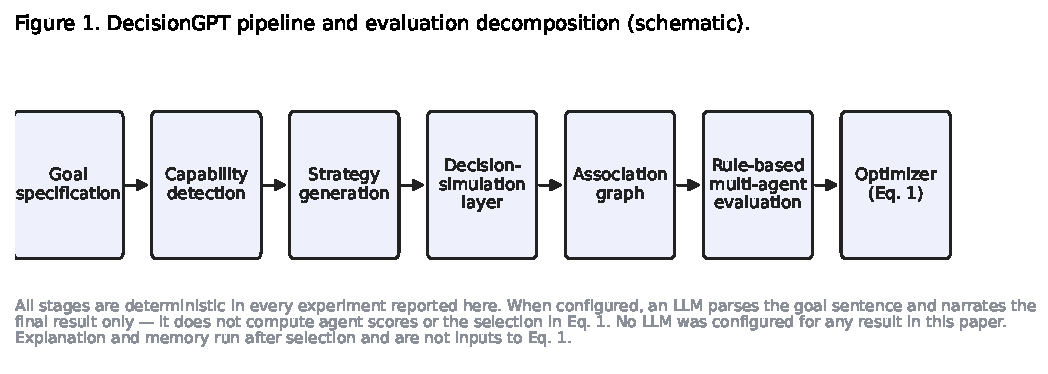
\includegraphics[width=\textwidth]{figure1_architecture.pdf}
\caption{DecisionGPT pipeline and evaluation decomposition (schematic). Goal
specification $\rightarrow$ capability detection $\rightarrow$ strategy
generation $\rightarrow$ decision-simulation layer $\rightarrow$ association
graph $\rightarrow$ rule-based multi-agent evaluation $\rightarrow$ optimizer
(Eq.~\ref{eq:opt}). All stages are deterministic in every experiment reported
here; when configured, an LLM parses the goal sentence and narrates the final
result only and does not compute agent scores or the selection in
Eq.~\ref{eq:opt} (no LLM was configured for any result in this paper).
Explanation and memory run after selection and are not inputs to
Eq.~\ref{eq:opt}. Schematic; no data.}
\label{fig:arch}
\end{figure*}

DecisionGPT is a capability-gated pipeline (Fig.~\ref{fig:arch}). Given a
natural-language goal and an uploaded dataset, it produces a ranked
recommendation with an internal confidence value and a post-hoc explanation. The
stages are:

\begin{enumerate}
\item \textbf{Goal specification.} A goal sentence is parsed into an objective
(e.g. increase revenue, increase profit, increase sales), a primary KPI, a
target percentage, and constraints. When an LLM is configured it performs this
parse and the final narration only; every parsed field is re-validated against
the data. All results in this paper were produced with no LLM configured
(Section~\ref{sec:evidence}).
\item \textbf{Capability detection.} The system checks whether the uploaded
data supports the requested objective. If required data is absent it returns an
explicit insufficient-evidence result rather than a fabricated value.
\item \textbf{Strategy generation.} Goal-templated candidate strategies
(pricing, marketing, inventory levers) are generated, gated by detected
capabilities.
\item \textbf{Business decision-simulation layer.} For each candidate, a
recursive forecast projects the KPI forward and an extrapolation-risk heuristic
scores how far the candidate's input values lie outside the historically
observed range. This layer is a \emph{digital model} in the sense of Kritzinger
et al.~\cite{Kritzinger2018}: it consumes manually loaded data and produces
offline projections with no automatic or bidirectional data flow.
\item \textbf{Evidence-labelled association graph.} Pairwise Granger tests over
the uploaded series build a directed graph whose edges carry heuristic evidence
labels (assumed / observational / data-supported / causally-validated). Edge
promotion is never automatic; in every experiment reported here the
causally-validated count is zero.
\item \textbf{Rule-based multi-agent evaluation.} Three deterministic agents ---
a business analyst, a financial advisor, and a risk manager --- score each
candidate in $[0,1]$. A fixed two-round structured exchange allows agents to
revise scores. Agent scores are computed by rules, not by an LLM.
\item \textbf{Strategy optimizer.} Candidates are ranked by
\begin{equation}
s \;=\; \frac{\mathrm{BA} + \mathrm{FA}}{2} \;-\; \lambda\,(1 - \mathrm{RM}),
\label{eq:opt}
\end{equation}
where $\mathrm{BA},\mathrm{FA},\mathrm{RM}\in[0,1]$ are the business-analyst,
financial-advisor, and risk-manager scores and $\lambda$ is the risk-penalty
weight. The production configuration (denoted \textbf{D0}) uses $\lambda=1$ and
no learned risk model (\code{risk\_model = None}), abbreviated \textbf{R0/D0}.
\item \textbf{Explanation and memory.} A post-hoc narration is generated from
the stored components; the decision and any later outcome are written to a
memory store. Neither stage feeds back into the selection
in~\eqref{eq:opt}.
\end{enumerate}

The confidence value is a fixed product of internal factors (inter-agent
agreement, a risk factor, an evidence factor, and an uncertainty penalty). It is
reproducible from stored components but is \emph{not} calibrated against any
human or outcome notion of confidence; we call it the \emph{internal confidence}.

%==============================================================================
\section{Experimental Design}
\label{sec:design}

\paragraph{Configurations}
The architecture comparison evaluates four cumulative configurations on
identical inputs: \textbf{A} --- prediction only (forecast, no strategy
mechanism); \textbf{B} --- prediction $+$ business decision-simulation layer;
\textbf{C} --- B $+$ a single evaluation agent; \textbf{D} --- B $+$ the full
three-agent rule-based evaluation layer (the production architecture).

\paragraph{Scenario--seed design}
Twelve scenarios (Section~\ref{sec:data}) are each instantiated with five random
seeds (42--46), producing a procedurally generated business per (scenario,
seed). Every configuration is evaluated on the identical generated business, so
observations are \emph{paired} per (scenario, seed): $12\times 5 = 60$ paired
observations per configuration. The ablation (Section~\ref{sec:ablation}) uses
the same 60-pair design across six configurations (full, and full minus each of
five components).

\paragraph{Pre-registration}
The risk-recalibration study (Section~\ref{sec:recal}) fixed its formula, its
variant set, its $\lambda$-selection rule, and seven acceptance criteria before
any recalibration run, following registered-report discipline~\cite{Nosek2018}.
The primary architecture comparison and ablation use the aggregation and testing
procedure specified in Section~\ref{sec:stats}.

\paragraph{Candidate-space fairness control}
An initial version of the strategy generator omitted a price-increase lever for
revenue and sales objectives, so the simulation layer's preferred candidate was
sometimes unavailable to the agent layer. We added the lever, verified that the
fraction of (scenario, seed) pairs whose simulation-preferred strategy is
present in the agent layer's candidate set rose from $0.333$ to $0.833$
(missing-when-supported rate $0.500 \rightarrow 0.000$), and re-ran the
architecture comparison, ablation, and diagnostic. The corrected runs are
byte-identical in every aggregate, confidence interval, and $p$-value to the
pre-correction runs (Section~\ref{sec:candspace}). All results in this paper use
the corrected runs.

\paragraph{Determinism and provenance}
Every experiment uses seed 42 for its non-scenario randomness, is recorded as a
completed run in the manifest with an identifier, dataset version, and model
versions, and asserts that the active model set is unchanged before and after.

%==============================================================================
\section{Data and Scenario Construction}
\label{sec:data}

\subsection{Designed scenarios (primary evidence)}
The twelve scenarios are \emph{deliberately constructed, not sampled} from a
population of businesses (Table~\ref{tab:scenarios}). Each fixes an industry
label, a primary decision lever, an objective, a primary KPI, and a target. They
span pricing, marketing, inventory, and conservative levers across apparel,
electronics, grocery, furniture, e-commerce, consumer-goods, regional-retail,
and small-manufacturing labels.

\begin{table*}[!t]
\caption{Designed evaluation scenarios. Primary evidence (configuration).
Synthetic, designed not sampled. Each scenario is instantiated with seeds
42--46. S04 and S07 use a documented revenue proxy for their primary KPI
(Section~\ref{sec:metrics}).}
\label{tab:scenarios}
\centering
\renewcommand{\arraystretch}{1.15}
\begin{tabular}{@{}llllll@{}}
\toprule
ID & Label & Lever & Objective & Primary KPI & Target\\
\midrule
S01 & Clothing retail --- revenue via pricing   & pricing      & increase revenue        & revenue                       & 12\%\\
S02 & Clothing retail --- profit via pricing    & pricing      & increase profit         & profit                        & 12\%\\
S03 & Electronics retail --- sales via marketing& marketing    & increase sales          & orders                        & 15\%\\
S04 & Grocery retail --- inventory risk         & inventory    & reduce inventory risk   & inventory risk (revenue proxy)& 10\%\\
S05 & Furniture retail --- high-ticket profit   & pricing      & increase profit         & profit                        & 15\%\\
S06 & E-commerce --- revenue via marketing      & marketing    & increase revenue        & revenue                       & 20\%\\
S07 & Apparel e-commerce --- marketing ROI      & marketing    & improve marketing ROI   & marketing ROI (revenue proxy) & 15\%\\
S08 & Consumer goods --- thin-margin profit     & inventory    & increase profit         & profit                        & 10\%\\
S09 & Regional retail --- price-sensitive sales & pricing      & increase sales          & orders                        & 12\%\\
S10 & Small manufacturing --- cost / profit     & inventory    & increase profit         & profit                        & 8\%\\
S11 & Mixed retail --- revenue via marketing    & marketing    & increase revenue        & revenue                       & 15\%\\
S12 & Small e-commerce --- conservative revenue & conservative & increase revenue        & revenue                       & 8\%\\
\bottomrule
\end{tabular}
\end{table*}

\paragraph{KPI proxy (S04, S07)}
Two objectives --- \code{reduce\_inventory\_risk} (S04) and
\code{improve\_marketing\_roi} (S07) --- have no directly simulated KPI pair.
For these, attainment of the scenario's revenue movement is used as a documented
proxy for \code{goal\_achievement}. These two scenarios are flagged in every
trace and are excluded in a robustness analysis
(Section~\ref{sec:robustness}). Their \code{goal\_achievement} values are
\emph{not} genuine revenue-outcome observations.

\subsection{Supporting datasets}
\begin{itemize}
\item \emph{Platform forecasting} (\code{platform-forecasting-v1}),
synthetic-controlled: forecasting sub-component evaluation (265 test rows, 1
seed). Not used for any real-world forecasting claim.
\item \emph{Platform churn} (\code{platform-churn-v1}), synthetic-controlled:
classification sub-component evaluation. Not used for any real-world churn claim.
\item \emph{Synthetic causal ground truth}, synthetic-controlled: method
validation of Granger recovery against a known graph. Not used for any real
causal claim.
\item \emph{India e-commerce orders} (Benroshan,
\code{external-india-ecommerce-v1}), real, \textbf{provenance unverified}:
descriptive analytics; a small forecasting reference (51 test days); a real-data
risk-ordering probe (23 derived price sub-series, 184 rows). Not used for
Table~\ref{tab:table2} evidence, for any representativeness or population claim,
or for unit-price/elasticity analysis (price is derived as revenue $\div$ units).
\item \emph{India festival calendar; policy repo-rate series}~\cite{RBIDBIE},
public context: optional exogenous covariates. Not used as targets or causal
evidence.
\item \emph{AGMARKNET agricultural wholesale prices}~\cite{AGMARKNET},
agricultural price: \emph{data pending} (not retrieved); integration present.
Not SME retail data; not used in any result here.
\item \emph{Real Indian SME decision outcomes}, own category:
Table~\ref{tab:table2} becomes available at $\geq 5$ matched records ---
\textbf{0 records; nothing now}.
\end{itemize}
Categories are never averaged. The Benroshan raw file (which contains customer
first names) is excluded from every committed processed artifact.

%==============================================================================
\section{Evaluation Metrics}
\label{sec:metrics}

\begin{itemize}
\item \textbf{Simulated goal achievement} --- attainment of a scenario's own
primary KPI computed from a simulated strategy output, in $[0,1]$. For
revenue/profit/orders objectives it is the realised fraction of the target
movement; for S04 and S07 it uses the revenue proxy above. It is a
model-internal construct on a procedurally generated business, \emph{not}
realised business value.
\item \textbf{Simulated risk-discounted benefit} --- the projected benefit
multiplied by one minus the simulation layer's extrapolation-risk score. It is
dominated by the extrapolation-risk heuristic and can be negative even when the
raw KPI movement is positive.
\item \textbf{Internal confidence} --- the fixed product of internal factors
described in Section~\ref{sec:arch}; reproducible from stored components, not
human-calibrated.
\item \textbf{Latency} --- wall-clock seconds per decision.
\item \textbf{Forecasting} --- mean absolute error (MAE), root-mean-square
error (RMSE), and, where actuals are non-degenerate, mean absolute percentage
error (MAPE).
\item \textbf{Classification (churn)} --- precision, recall, F1, and area under
the ROC curve (ROC-AUC). We do not report or refer to ``accuracy'' for these
models.
\item \textbf{Causal recovery} --- precision, recall, F1, and structural
Hamming distance (SHD) against a known synthetic graph.
\end{itemize}

%==============================================================================
\section{Statistical Analysis}
\label{sec:stats}

\paragraph{Descriptive aggregation}
For each configuration and metric we report the sample mean, median, and
standard deviation (Bessel-corrected), and a Student-$t$ 95\% interval on the
mean, $\text{mean} \pm t_{0.975,\,n-1}\, s/\sqrt{n}$. Because the scenarios are
\emph{designed rather than sampled}, this interval describes sampling
variability \emph{within the designed scenario suite}, not a
population~\cite{Shadish2002,Wasserstein2016}.

\paragraph{Paired comparison}
For each primary contrast we take per-(scenario, seed) differences
$d_i = x_i - y_i$ and report: the paired sample size $n$; the number of non-zero
differences $\Nnz$ (tolerance $10^{-9}$); the mean and median paired difference;
the count of pairs favouring each side (wins / ties / losses); the Wilcoxon
signed-rank statistic and two-sided $p$-value (\code{zero\_method = "wilcox"}, no
continuity correction); the $\rzn$ effect size with $Z = \Phi^{-1}(p/2)$
\cite{Fritz2012}; and the matched-pairs rank-biserial correlation as the
proportion of favourable minus unfavourable non-tied pairs~\cite{Kerby2014}. We
lead with the mean paired difference as the interpretable magnitude and never
report $r$ alone~\cite{Wasserstein2016}. When all paired differences are exactly
zero the test is not defined and we state ``significance not assessed'' rather
than reporting a $p$-value.

\paragraph{On the effect size $\rzn$}
This quantity is a monotone transform of the $p$-value and $\Nnz$; it is
retained for traceability with the frozen records but is \emph{not} an
independent effect-size estimate. Where $\Nnz$ is small
(Sections~\ref{sec:esize} and~\ref{sec:recal}) it saturates near 1 merely
because the few non-tied pairs agree in sign; we therefore also give the
rank-biserial correlation and, for the primary contrast, a bootstrap interval.

\paragraph{Clustering}
The 60 paired observations per configuration derive from 12 scenario generators
crossed with 5 seeds; observations within a generator are \emph{not
independent}. We therefore also report a scenario-level analysis that treats
each scenario's mean as one unit ($n = 12$) for the primary contrast
(Section~\ref{sec:robustness}), and we do not interpret any interval as
population inference.

\paragraph{Bootstrap interval (primary contrast only)}
From the 60 stored per-(scenario, seed) differences for $D - B$ we draw
$20{,}000$ paired bootstrap resamples (seed 42) and report the 2.5--97.5
percentile interval of the resampled mean. This is a re-analysis of frozen
observations, not a new experiment.

%==============================================================================
\section{Primary Results}
\label{sec:results}

\subsection{Architecture comparison}
\label{sec:archcmp}
Experiment \expid{0e1bd8dc}, $N = 60$ per configuration. Table~\ref{tab:arch},
Table~\ref{tab:paired}, and Fig.~\ref{fig:primary} report this comparison.

\begin{table*}[!t]
\caption{Architecture comparison (simulated goal achievement). Primary,
confirmatory. Synthetic. Student-$t$ 95\% intervals describe within-suite
variability. Experiment \expid{0e1bd8dc}.}
\label{tab:arch}
\centering
\renewcommand{\arraystretch}{1.2}
\begin{tabular}{@{}lrrrlrrr@{}}
\toprule
Config. & Mean & Median & SD & 95\% CI & Risk-disc.\ ben. & Int.\ conf. & Lat.\ (s)\\
\midrule
A --- Prediction only        & 0.0000 & 0.000 & 0.0000 & $[0.0000,\,0.0000]$ & $0.00$      & n/a   & 0.151\\
B --- $+$ Decision Simulation& \textbf{0.4856} & 0.4584 & 0.3138 & $[0.4045,\,0.5666]$ & $2508.40$   & n/a   & 1.408\\
C --- $+$ single agent       & 0.0025 & 0.000 & 0.0057 & $[0.0010,\,0.0040]$ & $190.94$    & n/a   & 1.392\\
D --- Full ($+$ multi-agent) & \textbf{0.0844} & 0.000 & 0.2784 & $[0.0125,\,0.1564]$ & $-2614.83$  & 0.139 & 1.680\\
\bottomrule
\end{tabular}
\end{table*}

\begin{table*}[!t]
\caption{Paired contrasts. Primary, confirmatory. $\Nnz$ is the number of
non-zero paired differences. Experiment \expid{0e1bd8dc}.}
\label{tab:paired}
\centering
\renewcommand{\arraystretch}{1.2}
\begin{tabular}{@{}lrrrlrrrr@{}}
\toprule
Contrast & $n$ & $\Nnz$ & Mean diff & 95\% CI (Student-$t$) & W / T / L & Wilcoxon $p$ (2-sided) & $\rzn$ & Rank-bis.\\
\midrule
$D - A$ & 60 & 10 & \textbf{$+0.0844$} & $[0.0125,\,0.1564]$ & 10 / 50 / 0 & $0.0045$ & 0.899 & $+1.00$\\
$D - B$ & 60 & 45 & \textbf{$-0.4011$} & $[-0.4783,\,-0.3239]$ & 0 / 15 / 45 & $<10^{-4}$ (recomp. $4.8\times10^{-9}$) & 0.873 & $-1.00$\\
\bottomrule
\end{tabular}
\end{table*}

For $D - B$, a $20{,}000$-sample paired bootstrap of the mean (seed 42) gives
95\% interval $[-0.4769,\,-0.3265]$, in close agreement with the Student-$t$
interval. The simulation-only configuration B beats the full architecture on 45
of 60 paired observations and is beaten on none. The full architecture's
per-(scenario, seed) distribution has best $1.000$, worst $0.000$, median
$0.000$, SD $0.278$: it attains a non-zero simulated goal achievement in only
two of twelve scenarios.

\begin{figure*}[!t]
\centering
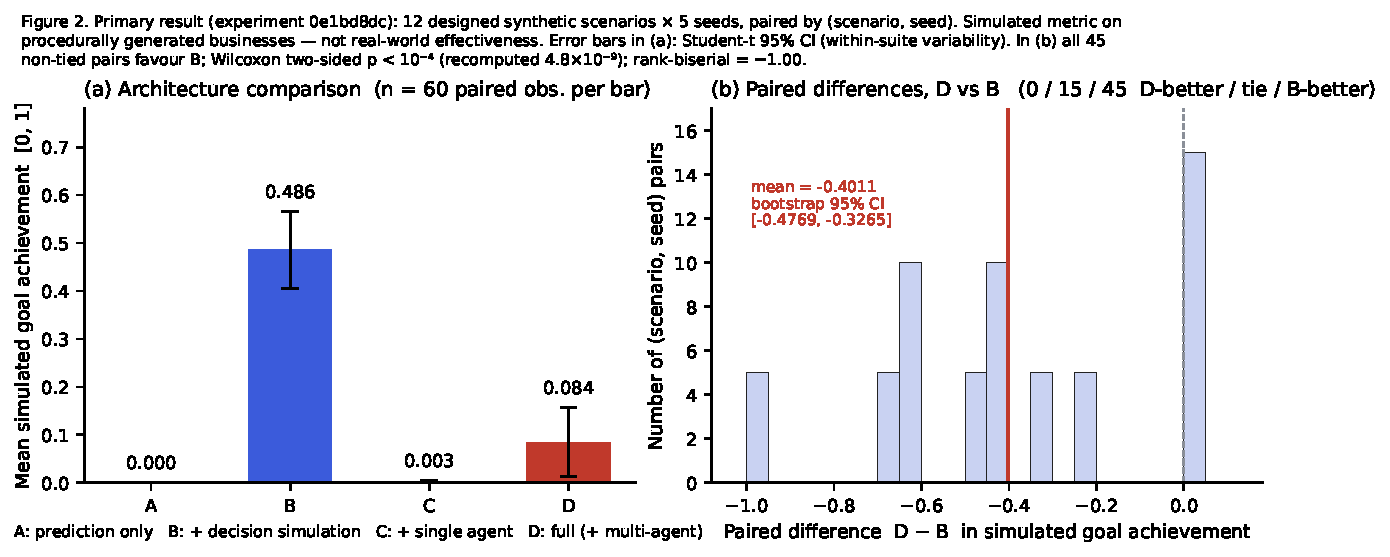
\includegraphics[width=\textwidth]{figure2_primary_comparison.pdf}
\caption{Primary result (experiment \expid{0e1bd8dc}). Twelve designed synthetic
scenarios $\times$ 5 seeds, paired by (scenario, seed); the metric is simulated
goal achievement on procedurally generated businesses and is not real-world
effectiveness. (a)~Mean simulated goal achievement for configurations
A~(prediction only), B~($+$ decision simulation), C~($+$ single agent),
D~(full, $+$ multi-agent); error bars are Student-$t$ 95\% intervals describing
within-suite variability ($n = 60$ per bar). The decision-simulation layer
raises the metric from $0.000$ to $0.486$; adding the rule-based multi-agent
layer reduces it to $0.084$. (b)~Distribution of the 60 per-(scenario, seed)
$D - B$ differences: all 45 non-tied pairs favour B, 15 are ties, none favour D.
The red line is the mean ($-0.401$); the bracket is the $20{,}000$-sample paired
bootstrap 95\% interval $[-0.4769,\,-0.3265]$. Wilcoxon two-sided $p < 10^{-4}$
(recomputed $4.8\times10^{-9}$); matched-pairs rank-biserial $= -1.00$ (a
boundary value reflecting sign-consistency, not practical size).}
\label{fig:primary}
\end{figure*}

\subsection{Interpretation of the effect sizes}
\label{sec:esize}
The $D - B$ rank-biserial correlation of $-1.00$ means only that all 45 non-tied
pairs point the same way (B better); it is a boundary value driven by
sign-consistency, not a statement of practical size. The \emph{interpretable
magnitude is the mean shift of $-0.401$ on a $[0,1]$ metric}, with a 95\%
interval excluding zero by a wide margin under both the Student-$t$ and bootstrap
methods. For $D - A$ only 10 of 60 pairs differ, so the $r = 0.90$ there should
likewise be read as ``the few non-tied pairs agree'', with the $+0.084$ mean
shift as the magnitude; D is above A only because A has no strategy mechanism at
all.

\subsection{Scenario-level analysis and robustness (RQ1, RQ2)}
\label{sec:robustness}
Treating each scenario's mean as one unit ($n = 12$), the $D - B$ difference is
negative in 9 scenarios, zero in 3 (S03, S09, S10 --- configurations tie because
both score 0 in S03/S09 and both score 1 in S10), and positive in none; the mean
scenario-level difference is $-0.401$ with a $20{,}000$-sample bootstrap 95\%
interval of $[-0.571,\,-0.235]$.

\emph{Excluding the two KPI-proxy scenarios (S04, S07)} --- a secondary analysis
of the frozen observations, not a new experiment --- leaves $n = 50$ paired
observations, wins/ties/losses $0/15/35$, mean paired difference $-0.3904$, and
Wilcoxon two-sided $p \approx 2.2\times10^{-7}$ (Fig.~\ref{fig:recal}b). The
headline degradation is therefore not an artefact of the revenue-proxy
scenarios.

\subsection{Candidate-space correction}
\label{sec:candspace}
The pre-correction architecture run (\expid{675cf17e}) and the post-correction
run (\expid{0e1bd8dc}) are byte-identical in every reported aggregate, interval,
and $p$-value, despite the candidate-coverage rate rising from $0.333$ to
$0.833$. The negative $D - B$ result is thus a scoring-rule effect, not a
consequence of the agent layer being unable to see the simulation layer's
preferred strategy.

\paragraph{Answering RQ1 and RQ2}
Within this controlled evaluation, the decision-simulation layer is the
component that carries the measurable objective value ($A \rightarrow B$ raises
the mean from $0.000$ to $0.486$); adding the implemented rule-based multi-agent
evaluation layer on top of it does not add value and significantly reduces the
simulated goal-achievement metric.

%==============================================================================
\section{Component Ablation}
\label{sec:ablation}

Experiment \expid{db58455b}, $N = 60$ per configuration. Table~\ref{tab:ablation}
and Fig.~\ref{fig:ablmech}(a) report this ablation.

\begin{figure*}[!t]
\centering
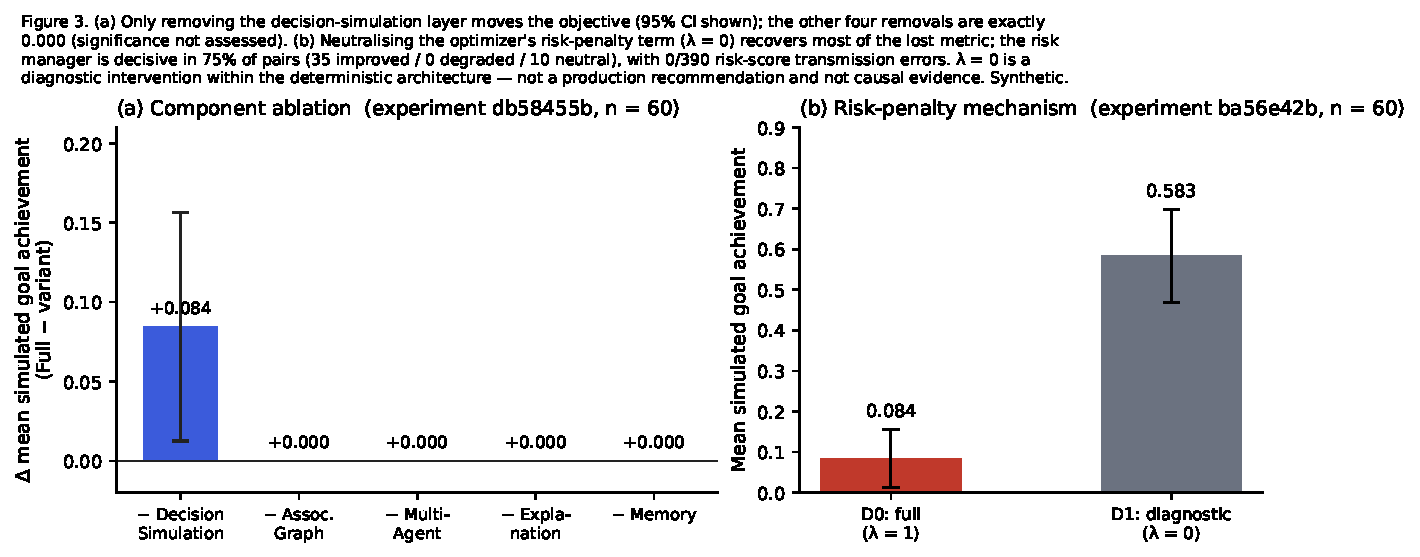
\includegraphics[width=\textwidth]{figure3_ablation_mechanism.pdf}
\caption{Component ablation and risk-penalty mechanism (sources \expid{db58455b},
\expid{ba56e42b}). (a)~Change in mean simulated goal achievement (Full $-$
variant, $n = 60$) for each removed component: only removing the
decision-simulation layer moves the objective ($+0.084$, 95\% CI
$[0.013,\,0.156]$, shown); removing the association graph, multi-agent layer,
explanation, or memory changes it by exactly $0.000$ (significance not assessed
--- all paired differences are zero). (b)~Mean simulated goal achievement for D0
(the full architecture, $\lambda = 1$) and D1 ($\lambda = 0$, the risk-penalty
term neutralised as a diagnostic); the risk manager is decisive in 75\% of pairs
(35 improved / 0 degraded / 10 neutral) with $0/390$ risk-score transmission
errors. $\lambda = 0$ is a diagnostic intervention within the deterministic
architecture --- not a production recommendation and not causal evidence about
real businesses; D1 also collapses the internal confidence value to $0.018$ and
is not a usable configuration. Synthetic scenarios throughout.}
\label{fig:ablmech}
\end{figure*}

\begin{table}[!t]
\caption{Component ablation. Primary, confirmatory. Synthetic. Experiment
\expid{db58455b}.}
\label{tab:ablation}
\centering
\renewcommand{\arraystretch}{1.25}
\begin{tabular}{@{}p{1.85cm}rrlr@{}}
\toprule
Configuration & Mean SGA & $\Delta$ vs Full & 95\% CI of $\Delta$ & Int.\ conf.\\
\midrule
Full                    & 0.0844 & ---      & ---                 & 0.139\\
$-$ Decision Simulation & \textbf{0.0000} & $+0.0844$ & $[0.0125,\,0.1564]$ & n/a\\
$-$ Association Graph    & 0.0844 & $0.0000$  & ---                 & 0.2512\\
$-$ Multi-Agent          & 0.0844 & $0.0000$  & ---                 & 0.1321\\
$-$ Explanation          & 0.0844 & $0.0000$  & ---                 & 0.139\\
$-$ Memory               & 0.0844 & $0.0000$  & ---                 & 0.139\\
\bottomrule
\end{tabular}

\vspace{2pt}
\footnotesize SGA $=$ simulated goal achievement.
\end{table}

For the decision-simulation removal, the paired contrast has $\Nnz = 10$,
wins/ties/losses $10/50/0$, Wilcoxon two-sided $p = 0.0045$. For the other four
removals \emph{every one of the 60 paired differences is exactly zero}, so
significance is not assessed.

\paragraph{Why the exact zeros are credible, not a null harness}
In the deterministic configuration the business-analyst and financial-advisor
scores are near-constant across candidates, so the strategy selected
by~\eqref{eq:opt} is governed by the single risk term. The association-graph,
multi-agent, explanation, and memory components feed only those near-flat
scores, the confidence value, or the post-hoc narration; none of them changes
which strategy~\eqref{eq:opt} selects, so the objective is unchanged to the
recorded precision. The one measurable non-simulation effect is that
\emph{removing the association graph raises the internal confidence value from
$0.139$ to $0.251$} without changing the selected strategy or the objective;
removing the multi-agent layer moves the internal confidence slightly to
$0.132$.

We do not conclude that these components are without value in general --- only
that, on this suite, under this deterministic configuration, they produce no
measurable change in the simulated goal-achievement metric.

%==============================================================================
\section{Mechanism and Risk Diagnosis}
\label{sec:mechanism}

Experiment \expid{ba56e42b}, 60 pairs / 390 strategy rows. This section is
\emph{controlled mechanism / diagnostic evidence within the implemented
deterministic architecture}. It is not causal inference and not real-world
evidence. We distinguish three things: a \emph{component ablation} removes a
module; a \emph{mechanism diagnosis} toggles one term inside a module and
measures the change on the same inputs; \emph{causal inference} would require
interventions in the world.

\paragraph{Isolating the risk-penalty term}
Let D1 denote the full architecture with the risk-penalty term in~\eqref{eq:opt}
un-weighted ($\lambda = 0$) while the risk manager still runs and still feeds the
confidence value. On the identical 60 (scenario, seed) pairs
(Fig.~\ref{fig:ablmech}(b)): simulated goal achievement mean
$0.0844\;[0.0125,0.1564]$ for D0 versus $\mathbf{0.5834}\;[0.4692,0.6976]$ for
D1; median $0.000$ versus $0.7582$; internal confidence $0.139$ versus
$\mathbf{0.0184}$; simulated risk-discounted benefit $-2614.83$ versus
$-2521.95$. Paired $D1 - D0$ on simulated goal achievement: $n = 60$,
$\Nnz = 35$, wins/ties/losses $35/25/0$, mean paired difference $\mathbf{+0.4989}$
(95\% CI $[0.3827,0.6152]$), Wilcoxon two-sided $p < 10^{-4}$, rank-biserial
$+1.00$.

\paragraph{Supporting checks}
(i)~Equation~\eqref{eq:opt} is verified to hold exactly on all 390 recorded
strategy rows (maximum deviation $0.0$). (ii)~The risk manager disagrees with
the simulation layer's preferred strategy on all 60 pairs. (iii)~Removing only
the risk-penalty term changes the selected strategy on 45 of 60 pairs
($75.0\%$): 35 of those changes improve the metric, 0 degrade it, 10 are
neutral. (iv)~There are 0 risk-score transmission errors in 390 rows --- the risk
manager faithfully passes through the simulation layer's extrapolation-risk
score; it is not independently mis-scoring.

\paragraph{Reading}
The intervention isolates the proximate mechanism \emph{within the deterministic
architecture}: the unbounded $-\lambda(1 - \mathrm{RM})$ term, acting on an
extrapolation-risk heuristic that is large for modest price moves because the
generated histories hold price nearly constant, drives the optimizer away from
the simulation layer's preferred strategy. It does \emph{not} establish a
real-world mechanism, and D1 is \emph{not} a usable configuration: it removes
risk management entirely, collapses the internal confidence value to $0.018$,
and leaves the simulated risk-discounted benefit negative. \textbf{Answering
RQ3:} the degradation is a scoring-rule interaction between near-flat agent
scores and an unbounded, mis-scaled risk penalty.

%==============================================================================
\section{Risk-Heuristic Recalibration (supplementary)}
\label{sec:recal}

Experiment \expid{b8516eef}. This is a \emph{pre-registered} study (formula,
seven variants, $\lambda$-selection rule, and seven acceptance criteria fixed
before running). It is \emph{supplementary}; production is unchanged.
Table~\ref{tab:recal} and Fig.~\ref{fig:recal}(a) report the variants.

\begin{figure*}[!t]
\centering
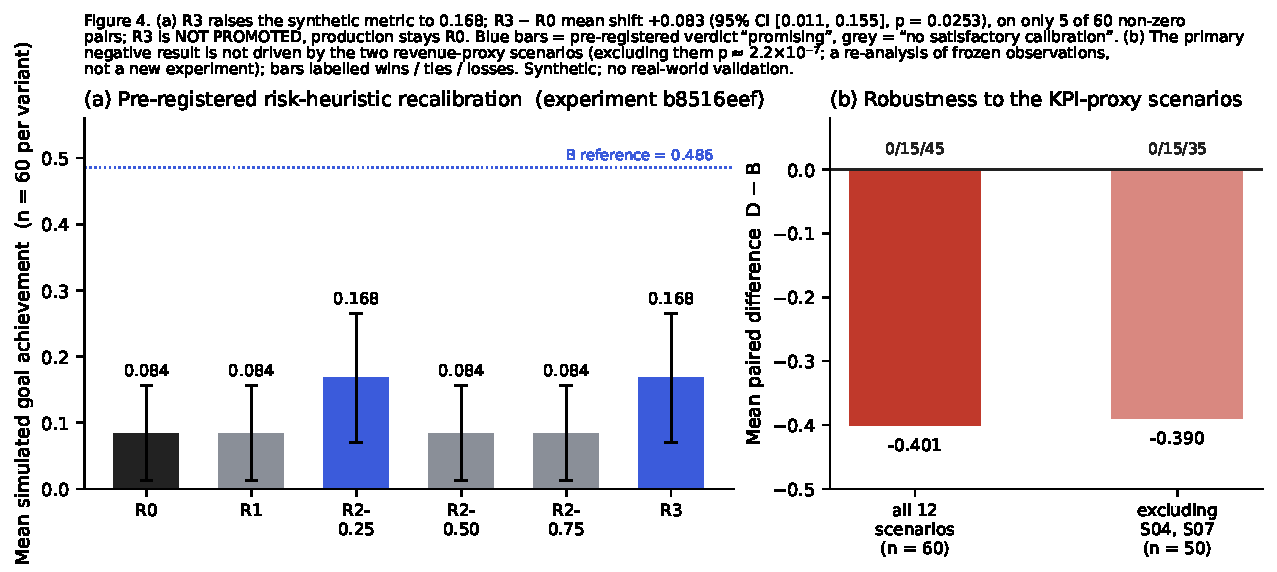
\includegraphics[width=\textwidth]{figure4_risk_calibration.pdf}
\caption{Pre-registered risk-heuristic recalibration and robustness (sources
\expid{b8516eef}, \expid{0e1bd8dc}). (a)~Mean simulated goal achievement ($n =
60$ per variant, Student-$t$ 95\% intervals) for R0~(production), R1, R2-0.25,
R2-0.50, R2-0.75, R3; blue bars carry the pre-registered verdict ``promising'',
grey ``no satisfactory calibration''; the dotted line is the decision-simulation
reference (B $= 0.486$). $R3 - R0$ mean shift $+0.083$ (95\% CI
$[0.011,\,0.155]$, $p = 0.0253$) on only 5 of 60 non-zero pairs; R3 is not
promoted and production stays R0. (b)~The primary $D - B$ mean paired difference
on all 12 scenarios ($-0.401$) and excluding the two revenue-proxy scenarios S04
and S07 ($-0.390$); bars are labelled wins / ties / losses. Excluding S04/S07
gives Wilcoxon two-sided $p \approx 2.2\times10^{-7}$ --- a re-analysis of the
frozen observations, not a new experiment. Synthetic; no real-world validation.}
\label{fig:recal}
\end{figure*}

\begin{table*}[!t]
\caption{Risk-heuristic recalibration variants. Supplementary, pre-registered.
Synthetic. \expid{R0} is the production configuration. Experiment
\expid{b8516eef}.}
\label{tab:recal}
\centering
\renewcommand{\arraystretch}{1.25}
\begin{tabular}{@{}llrlrrl@{}}
\toprule
Variant & Definition & Mean SGA & 95\% CI & Risk-disc.\ ben. & Int.\ conf. & Pre-registered verdict\\
\midrule
R0        & production (\code{extrapolation\_range} scale, $\lambda=1$) & 0.0844 & $[0.0125,\,0.1564]$ & $-2614.83$ & 0.139  & baseline\\
R1        & robust (MAD-based) scale only                              & 0.0844 & $[0.0125,\,0.1564]$ & $-2263.03$ & 0.1414 & no satisfactory calibration\\
R2-0.25   & bounded penalty weight $\lambda=0.25$ only                  & 0.1678 & $[0.0708,\,0.2647]$ & $-2614.83$ & 0.1087 & promising\\
R2-0.50   & $\lambda=0.50$ only                                        & 0.0844 & $[0.0125,\,0.1564]$ & $-2614.83$ & 0.139  & no satisfactory calibration\\
R2-0.75   & $\lambda=0.75$ only                                        & 0.0844 & $[0.0125,\,0.1564]$ & $-2614.83$ & 0.139  & no satisfactory calibration\\
\textbf{R3} & robust scale $+\ \lambda=0.25$                          & \textbf{0.1678} & $[0.0708,\,0.2647]$ & $\mathbf{+40.50}$ & 0.1087 & \textbf{promising --- not promoted}\\
\bottomrule
\end{tabular}

\vspace{2pt}
\footnotesize SGA $=$ simulated goal achievement.
\end{table*}

Paired \textbf{$R3 - R0$} on simulated goal achievement: $n = 60$,
$\mathbf{\Nnz = 5}$, wins/ties/losses $\mathbf{5/55/0}$, mean paired difference
$\mathbf{+0.083}$ (95\% CI $[0.0113,0.1553]$), Wilcoxon two-sided
$p = \mathbf{0.0253}$, $\rzn = 1.00$, rank-biserial $+1.00$. Only 5 of 60 pairs
change; the $r = 1.00$ reflects that those five agree in sign, and the
interpretable magnitude is the $+0.083$ mean shift. R3 closes approximately
21\% of the D0 $\rightarrow$ B gap in simulated goal achievement
$[(0.1678 - 0.0844)/(0.4856 - 0.0844)]$.

\paragraph{Real-data probe (experiment \expid{70617412})}
On the Benroshan implied-price data (23 derived sub-series, 184 rows,
price-variance regimes: 3 low / 11 moderate / 9 high), the production scale (R0)
and the robust scale (R1) produce \emph{identical} extrapolation-risk scores on
all 184 rows; Spearman $\rho$ between move-distance and risk is $0.9892$ for
both; there are 0 monotonicity violations for both; and $82.2\%$ of the 45
extreme out-of-range probes remain penalised at or above the $0.15$ threshold
under R1. The low-variance degeneracy that R3 targets \emph{does not occur} on
this real series (a real implied-price series spans a wide min--max, so the R0
denominator never collapses), so R3's central benefit could not be assessed
there. A single materialised business (307 daily observations, treated as one
unit --- no inferential test) selects the same strategy under every variant.

\paragraph{Verdict}
R3 improves the synthetic metric on a small minority of pairs; the effect is
\emph{not validated on real Indian SME data}; R3 is \emph{not promoted}; the
production configuration remains R0/D0. This is a pre-registered diagnosis, not a
validated improvement.

%==============================================================================
\section{Predictive Supporting Results}
\label{sec:predictive}

These are \emph{supporting predictive benchmarks on synthetic evaluation data},
single-seed point estimates with no confidence intervals and no significance
tests. They are not the contribution and imply nothing about business
performance. We do not use the term ``accuracy''.

\begin{table}[!t]
\caption{Forecasting sub-component --- synthetic-controlled
(\code{platform-forecasting-v1}, 265 test rows, seed 42). Supporting; point
estimates.}
\label{tab:forecast}
\centering
\renewcommand{\arraystretch}{1.2}
\begin{tabular}{@{}lrrr@{}}
\toprule
Model & MAE & RMSE & MAPE\\
\midrule
Naive   & 24.6597 & 38.2751 & 15.4647\%\\
Linear  & 17.2913 & 25.5112 & 12.4894\%\\
XGBoost & 15.1389 & 21.8631 & 10.2969\%\\
\bottomrule
\end{tabular}
\end{table}

\begin{table}[!t]
\caption{Classification (churn) sub-component --- synthetic-controlled
(\code{platform-churn-v1}, seed 42). Supporting; point estimates.}
\label{tab:churn}
\centering
\renewcommand{\arraystretch}{1.2}
\begin{tabular}{@{}lrrrr@{}}
\toprule
Model & Precision & Recall & F1 & ROC-AUC\\
\midrule
Logistic regression & 0.7076 & 0.6337 & 0.6686 & 0.7978\\
Random forest       & 0.7125 & 0.6172 & 0.6614 & 0.7928\\
XGBoost             & 0.6990 & 0.6209 & 0.6576 & 0.7922\\
\bottomrule
\end{tabular}
\end{table}

For the real, provenance-unverified Benroshan series (51 test days): Naive
MAE $19.92$ / RMSE $31.25$; Linear $18.47$ / $28.51$; XGBoost $15.27$ / $23.89$.
\textbf{MAPE is omitted}: the series has zero-sales days, on which MAPE is
degenerate (observed $110$--$276\%$)~\cite{Hyndman2006}. This is a single small
series, reported descriptively, with no significance and no representativeness
claim.

\paragraph{Causal-recovery method validation (experiment \expid{36d0d404})}
Against a known synthetic graph ($A\!\rightarrow\!B\!\rightarrow\!C$ at lag 1;
$D$ an independent noise series), pairwise Granger recovery with maximum lag 3
and \emph{no multiple-comparison correction} gives precision $0.40$, recall
$1.00$, F1 $0.571$, SHD $3$ (true positives $A\!\rightarrow\!B$,
$B\!\rightarrow\!C$; false positives $A\!\rightarrow\!C$, $B\!\rightarrow\!A$,
$D\!\rightarrow\!B$; no false negatives). This validates the \emph{recovery
method} against a known structure only. It does not establish any real-world
causal relationship; the false positives are the expected transitive and
reverse edges of a weak pairwise method~\cite{Spirtes2000,Benjamini1995,Granger1969},
and the deployed system's causally-validated edge count is 0.

%==============================================================================
\section{Evidence Boundaries and Real-World Readiness}
\label{sec:evidence}

The following are reported as \emph{results}, not caveats
(Table~\ref{tab:boundaries}).

\begin{table}[!t]
\caption{Evidence boundaries. Reported as results.}
\label{tab:boundaries}
\centering
\renewcommand{\arraystretch}{1.25}
\begin{tabular}{@{}p{5.0cm}p{2.6cm}@{}}
\toprule
Evidence & Status\\
\midrule
Real SME decision outcomes            & \textbf{0} records\\
Matched prediction evaluations        & \textbf{0} records\\
Real-world decision-outcome validation (Table~\ref{tab:table2}) & \textbf{NOT READY}\\
Real-LLM evaluation                   & \textbf{BLOCKED}\\
Human / user study                    & not conducted\\
Real interventional causal evidence   & \textbf{0}; \code{CAUSALLY\_VALIDATED = 0}\\
Business ROI / financial-impact evidence & none\\
External / commercial system baseline & none\\
\bottomrule
\end{tabular}
\end{table}

\begin{table}[!t]
\caption{Real-world decision-outcome validation: \textbf{NOT READY}. No real SME
decision outcomes or matched post-decision observations were available at the
time of evaluation (readiness threshold $\geq 5$ genuine matched records;
current count 0). No result is reported and no synthetic or simulated
observation is substituted.}
\label{tab:table2}
\centering
\renewcommand{\arraystretch}{1.2}
\begin{tabular}{@{}llcccc@{}}
\toprule
Decision ID & Strategy & Predicted & Actual & Error & \% error\\
\midrule
\multicolumn{6}{c}{\emph{no rows --- 0 real matched outcomes; collection is future work}}\\
\bottomrule
\end{tabular}
\end{table}

\paragraph{Real LLM}
No LLM provider was configured (\code{llm\_enabled = false}, provider and model
both empty). The implemented multi-agent result is a \textbf{rule-based
deterministic evaluation}, not an LLM experiment. We do not report LLM outputs,
prompts, token counts, latency, or judge scores, and we make no claim about how
a real LLM would behave. A frozen real-LLM evaluation protocol exists as future
validation infrastructure; the LLM, when configured, affects goal parsing and
final narration only, not the agent scores or the selection in~\eqref{eq:opt}.

%==============================================================================
\section{Discussion}
\label{sec:discussion}

\paragraph{What the study establishes}
Under a controlled, paired, pre-registered evaluation on 12 designed scenarios
and 5 seeds, the business decision-simulation layer is the only component that
raises the simulated goal-achievement metric, and adding the implemented
rule-based multi-agent evaluation layer on top of it reduces that metric ---
across the paired evaluation, with 45 of 60 paired observations worse and none
better, robust to excluding the two KPI-proxy scenarios and to a scenario-level
analysis, and unchanged by a candidate-space correction. The proximate
mechanism, within the deterministic architecture, is the optimizer's unbounded
risk-penalty term operating on near-flat agent scores and a mis-scaled
extrapolation-risk heuristic.

\paragraph{What the study does not establish}
It does not establish that multi-agent reasoning or debate is generally harmful;
that an LLM-based agent implementation would behave the same way; that
DecisionGPT is ineffective for real SMEs; that the architecture would fail in
production; that the findings generalise to arbitrary businesses; or that real
business outcomes would decline. All decision evidence is synthetic and
scenario-based, the agents are deterministic rule-based scorers, the second
exchange round is inert in this mode, and there are zero real outcomes.

\paragraph{Why the negative result is useful}
Component-level evaluation surfaces a concrete, reproducible interaction ---
near-flat agent scores, the fixed optimizer rule, and an unbounded risk-penalty
term --- that an aggregate ``does the system work'' evaluation would hide. The
result is consistent with a broader literature finding that added agent layers
do not reliably help~\cite{Wang2024,Smit2024,Huang2024,Cemri2025} and extends
that literature to a decision-selection task with a simulator in the loop. It
also has a constructive reading for builders of such systems: a deterministic
simulation layer can be the load-bearing component, and a risk term added on top
of it should be bounded and scale-calibrated before more reasoning machinery is
layered on. Reporting the result, rather than filing it away, follows the norm
against publication bias toward positive findings~\cite{Rosenthal1979}.

\paragraph{Terminology}
Consistent with Kritzinger et al.~\cite{Kritzinger2018}, the simulation
component is a digital \emph{model}, not a data-integrated digital twin; the
graph component is an \emph{evidence-labelled association graph}, and we reserve
``causal'' for the synthetic method validation; the agents are \emph{rule-based}
scorers; and ``validated'' is used only where a frozen record supports it
(nowhere for real SMEs, R3, causality, or the LLM).

%==============================================================================
\section{Limitations}
\label{sec:limitations}

We state what each limitation constrains rather than apologise for it.
\begin{itemize}
\item \textbf{Synthetic-only decision evaluation.} Every
simulated-goal-achievement number is from a procedurally generated business.
Constrains: external validity; no statement about real decision quality follows.
\item \textbf{Designed, not sampled, scenarios ($n = 12$).} Constrains: no
population inference; the Student-$t$ and bootstrap intervals describe
within-suite variability only.
\item \textbf{Five seeds per scenario; clustered observations.} Constrains: the
60 paired observations are not independent; the scenario-level analysis
($n = 12$) is the conservative reading.
\item \textbf{Deterministic template-mode agents; inert second round.}
Constrains: the multi-agent finding is scoped to this configuration; an
LLM-based implementation is untested and could differ.
\item \textbf{No external system baseline.} Constrains: no superiority or
comparative claim; the contribution is component isolation within one
architecture.
\item \textbf{Two revenue-proxy scenarios (S04, S07).} Constrains: their
\code{goal\_achievement} values are not genuine revenue outcomes; the robustness
analysis excluding them is provided.
\item \textbf{Bounded, endpoint-heavy objective.} Constrains:
\code{goal\_achievement} has mass at 0 and 1; the median of the full
architecture's distribution is 0; $t$-based intervals are supplemented with a
bootstrap for the primary contrast.
\item \textbf{Low statistical power in secondary comparisons.} $D - A$ and
$R3 - R0$ have only 10 and 5 non-zero pairs; their $r$ values are near-boundary
and the mean shift is the interpretable quantity.
\item \textbf{Zero real SME outcomes; Table~\ref{tab:table2} NOT READY.}
Constrains: no real-world predictive-accuracy or effectiveness result exists.
\item \textbf{Real-LLM evaluation BLOCKED.} Constrains: no claim about LLM-agent
behaviour.
\item \textbf{No human evaluation.} Constrains: no explainability, comprehension,
or usability claim.
\item \textbf{No real interventional causal evidence
(\code{CAUSALLY\_VALIDATED = 0}).} Constrains: the causal component is method
validation on synthetic ground truth only.
\item \textbf{Single real dataset, provenance unverified, one business.}
Constrains: the real-data risk probe is descriptive with no inferential test.
\item \textbf{Robust-scale limitations.} The MAD-based scale in R1/R3 has low
Gaussian efficiency and assumes symmetry~\cite{Rousseeuw1993}; the $\lambda$ grid
($\{0.25, 0.50, 0.75\}$) is motivated but not exhaustively searched, by design.
\end{itemize}

%==============================================================================
\section{Reproducibility and Research Integrity}
\label{sec:repro}

\begin{itemize}
\item \textbf{Manifest.} 16 completed experiments, each with an identifier, seed
42, dataset version, and model versions;
\code{experiments/experiment\_manifest.json}, SHA-256
\code{94aa419c703b1babb465975463b26e55255755a7687ecbecadb6db4c4c15cbff}. The
primary results table is machine-readable in
\code{experiments/paper\_results\_snapshot.json} (four of five paper tables
ready; Table~\ref{tab:table2} not ready).
\item \textbf{Environment.} Python 3.12.0; the dependency set was corrected once
during preparation because the previously pinned stack was uninstallable (a
dependency required \code{numpy} $\geq 2$); a clean-room rebuild reproduced the
forecasting, churn, and causal-recovery numbers exactly.
\item \textbf{Determinism.} The aggregation functions are pure functions of the
stored observation arrays; re-running the aggregation on the same manifest
yields identical numbers. A unit test checks the aggregation against a
hand-computed mean/SD/interval and checks that the same (scenario, seed)
reproduces the same generated business.
\item \textbf{Production/research isolation.} The production decision path uses
the default configuration (\eqref{eq:opt} with $\lambda = 1$,
\code{risk\_model = None}, i.e. R0/D0). Every non-default configuration (D1, R1,
R2-$\lambda$, R3) is a research variant; no experiment promotes a model or
changes the production configuration.
\item \textbf{Data governance.} Five data categories (real,
synthetic-controlled, synthetic-context, public-context, agricultural-price) are
never averaged; real-SME-outcome material is admitted to Table~\ref{tab:table2}
only at $\geq 5$ genuine matched records; the real-LLM and causal-validation
states are held at \emph{BLOCKED} and \code{CAUSALLY\_VALIDATED = 0}.
\item \textbf{Historical documentation.} Some earlier internal reports carry
point-in-time counts from when they were written. The authoritative current
state --- 16 experiments and the current test total --- is recorded in the
manifest and the preparation report; the historical documents are preserved
rather than rewritten. No experiment value was changed to reconcile them.
\end{itemize}

\paragraph{Integrity statement}
No experiment was invented, re-run, re-seeded, or modified for this manuscript;
no scenario or score was changed; no real SME, customer, human-subject, or LLM
result was fabricated; Table~\ref{tab:table2} was not filled; R3 was not
promoted; and synthetic evidence was not relabelled as real. Where evidence is
unavailable, the paper says so.

%==============================================================================
\section{Future Work}
\label{sec:future}

\begin{itemize}
\item \textbf{Real SME decision-outcome collection.} A consent-gated,
provenance-checked, leakage-guarded import workflow exists; populating it to
$\geq 5$ matched records enables Table~\ref{tab:table2} and a real
predictive-accuracy evaluation.
\item \textbf{Real-LLM arm.} Run the frozen real-LLM protocol (identical inputs,
LLM agent scoring and narration only) and compare against the rule-based
configuration; account for LLM-evaluator bias~\cite{Zheng2023}.
\item \textbf{Repeated-seed intervals for the predictive sub-components} so
forecasting and churn can be reported with confidence intervals rather than
point estimates.
\item \textbf{A real interventional study} for any causal claim; until then the
graph remains an evidence-labelled association graph.
\item \textbf{A human study} of the explanation component (comprehension, trust,
decision quality).
\item \textbf{Broader and sampled scenarios}, including generators with
realistic price variation, to test whether the risk pathology is specific to
near-constant-price histories.
\item \textbf{An external-system comparison} to move beyond within-architecture
component isolation.
\end{itemize}

%==============================================================================
\section{Conclusion}
\label{sec:conclusion}

On a pre-registered, controlled evaluation of 12 designed scenarios and 5 seeds,
a deterministic business decision-simulation layer is the only component of an
integrated decision-support architecture that raises a simulated
goal-achievement metric, and adding a rule-based multi-agent evaluation layer on
top of it reduces that metric (mean shift $-0.401$; 45 of 60 paired observations
worse, none better; $p < 10^{-4}$), through an identified scoring-rule
interaction rather than an unequal strategy space. A pre-registered recalibration
of the risk heuristic is promising on the synthetic suite but inert on the one
real dataset and is not adopted. No real SME outcomes, real-LLM evaluation,
human study, or real causal evidence exists, and the paper makes no real-world
effectiveness, superiority, or generalisation claim. The contribution is a
reproducible component-level evaluation, a mechanism-diagnosed negative result
for the tested multi-agent configuration, and an evidence-boundary framework
that keeps controlled synthetic evidence separate from the real-world validation
that remains future work.

%==============================================================================
\section*{Reproducibility Artefacts}
The finalized source manuscript (\code{docs/PAPER\_DRAFT.md}), the reference
verification log (\code{docs/PAPER\_REFERENCES.md}), the figure render script and
its frozen input data (\code{docs/figures/make\_figures.py},
\code{docs/figures/figure\_data.json}), and a 66-point numerical-consistency
check of every value in this paper against the frozen manifest and snapshot are
in the project repository. No experiment was executed during the preparation of
this manuscript.

%==============================================================================
\bibliographystyle{IEEEtran}
\bibliography{references}

\end{document}
